\section{非惯性参考系和惯性力}\label{sec:12.01}

在上章中,我们指出规律的形式是绝对的,即对于所有的惯
性系,动力学方程的形式是一样的。本章讨论非惯性参考系的问
题。所谓非惯性系是指相对于惯性系作变速运动的参考系。在非
惯性系中,惯性定律及牛顿第二定律不再成立。例如,加速向前
开动的火车或汽车,就是个非惯性系。在车中,虽然没有看到任
何人或物推我们,但却会不由自主地向后倾倒。这种相对于车厢
的加速度是怎样来的呢?这是来自加速度的相对性。在第二章中
曾指出,如果物体$ A $对参考系$ K $为静止或匀速运动,有另一参考
系$ K' $相对于$ K $以加速度$ \vec{a}_0 $运动,则对$ K ' $而言,$ A $作加速运动,其
加速度为$ - \vec{a} _ { 0 } $,这就是向后倾倒的原因。在非惯性系中出现了不
与物体间作用力相联系的加速度,似乎说明了非惯性系对于讨论
动力学问题是复杂的、不恰当的,似乎说明我们永远不要选择这
种参考系来讨论力学问题。遗憾的是,在许多情况,我们不得不
选择这种“不恰当”的参考系,而且在实际工作中,这种“不恰
当”的参考系,却是最方便的参考系。地球往往是在实际工作中
不得不采用的参考系,而严格说来它是一个非惯性系。因而,讨
论有关非惯性系的特定问题,是非常必要的。

我们仍以匀加速运动的车厢为例,设其加速度为$ \vec{a} _ { 0 } $(图\ref{fig:12.01}。
% 352.jpg
\begin{figure}[h]
  \centering
  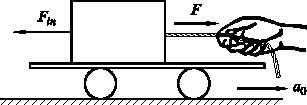
\includegraphics{figure/fig12.01}
  \caption{}
  \label{fig:12.01}
\end{figure}
如果物体$ A $相对于车厢的加速度为$ \vec{a}' $,则按加速度合成公式\eqref{eqn:02.04.05},
物体$ A $相对于地面参考系的加速度$ \vec{a} $为
\begin{equation}\label{eqn:12.01.01}
  \vec{a} = \vec{a} ^ { \prime } + \vec{a} _ { 0 }
\end{equation}
地面参考系近似于惯性参考系,牛顿第二定律成立,所以作用在
$ A $上的外力$ F $应为
\begin{equation*}
  \vec{F} = m \vec{a} = m \left( \vec{a} ^ { \prime } + \vec{a} _ { 0 } \right) = m \vec{a} ^ { \prime } + m \vec{a} _ { 0 }
\end{equation*}
其中$ m $为$ A $的质量。上式可以写成
\begin{equation}\label{eqn:12.01.02}
  m \vec{a} ^ { \prime } = \vec{P} - m \vec{a} _ { 0 }
\end{equation}
式\eqref{eqn:12.01.02}清楚地表明,在车厢参考系中,质量与加速度之积
$ m \vec{a} ' $并不等于作用力$\vec{F}$,相差值$ - m \vec{a} _ 0 $反映了车厢参考系的非惯
性性质。为了使得在车厢参照系中牛顿第二定律形式上仍然适
用,我们把$-m\vec{a}_0$设想为作用在物体上的一个力,称为惯性力,
写为
\begin{equation}\label{eqn:12.01.03}
  \vec{F} _ { in } = - m \vec{a} _ { 0 }
\end{equation}
这样,式\eqref{eqn:12.01.02}就可以写成
\begin{equation}\label{eqn:12.01.04}
  m \vec{a} ^ { \prime } = \vec{F} + \vec{F} _ {in}
\end{equation}
也就是说作用在物体上的总力,是真实的外力$\vec{F}$与设想的惯性力
$\vec{F}_{in}$之和。式\eqref{eqn:12.01.04}在形式上与牛顿第二定律是一样的。换言
之,在非惯性系中,若计及惯性力,那么,物体的运动依然满足
牛顿第二定律。如,当车加速时人会向后倾倒的现象,现在可
以解释为人受了惯性力$ \vec{F}_{in}=-m\vec{a}_0 $的作用,$\vec{F}_{in}$的方向与$\vec{a}_0$相反,
故人被向后拉。

引入了惯性力的概念,就使牛顿第二定律不仅适用于惯性
% 353.jpg
系,而且也适用于非惯性系。应该再次强调,惯性力$ \vec{F}_{in} $的来源
是参考系的非惯性性质,与电磁力、摩擦力等等物体之间的相
互作用是有区别的。从原则上说,只要我们选择惯性系,就可以
消除惯性力,而物体之间的真实作用力,是不能用这样的方法来
消除的。

我们看到,对于非惯性系,关键在寻找惯性力的正确表达
式,然后把真实力与惯性力的矢量和作为总力,就可以在非惯性
系中应用牛顿第一定律和第二定律来处理力学问题。关于第二定
律上面已经作了讨论。所调第一定律适用,是说当质点在某非惯
性系中所受总力(包括真实力和惯性力)为零时,对该非惯性系来
说,该质点静止或作匀速直线运动。而牛顿第三定律是讨论两个
物体间真实相互作用力的性质,惯性力是虚拟力,来源于参考系
的非惯性性质,并非物体之间的真实的相互作用,所以对非惯性
系来说,第三定律一般不再适用。

\begin{figure}[h]
  \vspace{1em}
  \centering
  \subfigure[\label{fig:12.02a}]{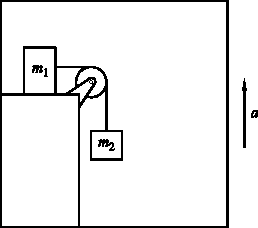
\includegraphics{figure/fig12.02a}}
  \subfigure[\label{fig:12.02b}]{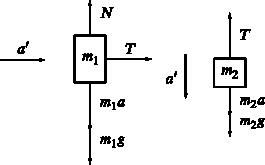
\includegraphics{figure/fig12.02b}}
  \caption{}
  \label{fig:12.02}
  \vspace{0.5em}
\end{figure}

\example 图\ref{fig:12.02a}中升降机内物体$ m _ { 1 } = 1 0 0 $克,$ m _ { 2 } = 2 0 0 $克,
用滑轮连接。升降机以加速度$ a = g / 2 = 4 . 9 $米/秒\textsuperscript{2}上升。求

(1) 在机内的观察者看到这两个物体的加速度是多少?

(2) 在机外地面上的观察者看到的加速度又是多少?

% 354.jpg
\solution (1) 在机内观察,因为升降机以加速度$\vec{a}$上升,故此系
统是非惯性系。惯性力是$ -m\vec{a} $。由图\ref{fig:12.02b}知各物体的动力学
方程为:
\begin{align*}
  \beforetext{\hspace{2em}对\ensuremath{m_2}有} & m _ { 2 } g + m _ { 2 } a - T = m _ { 2 } a ^ { \prime } \\
  \beforetext{\hspace{2em}对\ensuremath{m_1}有} & T = m _ { 1 } a ^ { \prime }
\end{align*}
\begin{equation*}
  N - m _ { 1 } g - m _ { 1 } a = 0
\end{equation*}
可解得
\begin{align*}
  N              & = \frac { 3 } { 2 } m _ { 1 } g                                      \\
                 & = 1 4 . 7 \times 1 0 ^ { 4 } \text{达因}                               \\
  a ^ { \prime } & = \frac { 3 m _ { 3 } g } { 2 \left( m _ { 1 } - m _ { 2 } \right) } \\
                 & = 9 . 8 \text{ 米/秒} ^ 2                                              \\
  T              & = m _ { 1 } a ^ { \prime }                                           \\
                 & = 9 . 8 \times 1 0 ^ { 4 } \text{ 达因}
\end{align*}

(2) 在地面上的观察者,是在惯性系中观察,不存在惯性力,
只是加速度的合成问题。各物体的动力学方程为
\begin{align*}
  \beforetext{\hspace{2em}对\ensuremath{m_2}有} & T - m _ { 2 } g = m _ { 2 } a _ { 2 } = m _ { 2 } \left( a - a ^ { \prime } \right) \\
  \beforetext{\hspace{2em}对\ensuremath{m_1}有} & T = m _ { 1 } a ^ { \prime }
\end{align*}
\begin{equation*}
  N - m _ { 1 } g = m _ { 1 } a
\end{equation*}
\begin{align*}
  \beforetext{解之得} N & = \frac { 3 } { 2 } m _ { 1 } g                                      \\
                     & = 1 . 4 7 \times 1 0 ^ { 4 } \text{ 达因}                              \\
  a ^ { \prime }     & = \frac { 3 m _ { 2 } g } { 2 \left( m _ { 1 } + m _ { 2 } \right) } \\
                     & = 9 . 8 \text{ 米/秒} ^ 2
\end{align*}
% 355.jpg
\begin{equation*}
  \begin{split}
    T &= m _ { 1 } a ^ { \prime } \\
    &= 9 . 8 \times 1 0 ^ { 4 } \text{ 达因} \\
    a _ { 2 } &= a - a ^ { \prime } \\[-0.5em]
    &= \frac { 1 } { 2 } g - \frac { 3 m _ { 2 } g } { 2 ( m _ { 1 } + m _ { 2 } ) } \\
    &= - 4 . 9 \text{ 米/秒} ^ 2 \\
    a _ { 1 } &= \sqrt { a ^ { 2 } + a ^ { \prime 2 } } \\
    &= 1 0 . 8 \text{ 米/秒} ^ 2 \\
    \theta &= \tg ^ { - 1 } \frac { 4 . 9 } { 9 . 8 } \\
    &= 2 6 ^ { \circ } 3 5 ^ { \prime }
  \end{split}
\end{equation*}
所以,在地面惯性系看来,$ m _ 2 $仍然是向着地面下落,但加速度是
$ a _ { 2 } = 4 . 9 $米/秒\textsuperscript{2},而不同于在非惯性参考系的升降机内所见到的加
速度$ a ^ { \prime } = 9 . 8 $米/秒\textsuperscript{2}。在地面观察,$ m_1 $不是象机内观察到的那样作
水平直线运动,而是沿与水平成夹角$ \theta = 2 6 ^ { \circ } 3 5 ^ { \prime } $的方向,作$ a _ { 1 } =
  10.8 $米/秒\textsuperscript{2}的匀加速运动。
